In this section, I will talk about the increase in complexity during embryonic development.
I will first try to define in complexity in an organism in general terms, mentioning alternative definitions that have been already proposed.
Then, I will explore the relations between complexity in evolution and development, and discuss the possibility of a trend in terms of complexity increase.


\subsection{Defining complexity}
Daniel W. McShea has provided an useful general definition of biological complexity. According to him, complexity is "the amount of differentiation among its parts or, where variation is discontinuous, the number of part types" \citep{McShea1996,McShea2015}.
This definition can be used at different hierarchical levels of biological organization, e.g., tissues, cells, genes.
Indeed, a measure of morphological complexity that has been favoured by some authors 
%(perhaps because of its intuitiveness), 
is the number of cell types that compose an organism 
	\citep{Valentine1994,Bell1997,Bonner2004}.
Importantly, with this definition, complexity at different levels are not necessarily correlated.

%These "parts" might be body segments (e.g., of an insect) or genes.
%It is evident that these definitions are problematic.
%It is doubtful to say that some centipede is more complex than a beetle, just based in the different number of segments they have.

This is related with the already acknowledged lack of correlation between the number of coding-genes and morphological complexity, 
%This lack of correspondence, 
sometimes referred as the "G-value paradox"
	\citep{Hahn2002}.
Some decades ago, there was the expectation that the morphological complexity should correlate with the number of genes in an organism. 
With the release of the first eukaryotic genome sequences, such correspondence was not observed.
Before that, the lack of correspondence between genome size and organism complexity (or "C-value paradox") was also noted.

An alternative definition of complexity includes not only the "number of parts" but also the "interaction among parts" 
	\citep{McShea1996,Arthur2010}.
This could be illustrated with the number of gene-gene interactions (e.g., expression regulation by a transcription factor binding to a promoter region of another gene),
such that when comparing two different organisms that have same number of genes, 
one organism could be considered to be more complex than the other if the former has more gene-gene interactions than the latter.

%This definition is also level-independent. 
%Again this definition is disputable, as it is acknowledged 
As before, a high complexity at the molecular level would not necessarily imply a high complexity at a higher level. 
Related to this is the observation that 
In fact, it is acknowledged that, during evolution, gene-gene interactions underlying a phenotype
can increase their complexity without affecting the phenotype 
	\citep{Muller1999,True2001,Salazar-Ciudad2009}.

%\subsection{Complexity as number of cells}

\subsection{Complexity Increase in Development}

The increase in complexity in an organism during embryogenesis is probably one of the most intuitive processes of animal development.

It is commonly seen even as one of its defining characteristics.
Eric H. Davidson described the progressive increase in complexity as the "essence" of development \citep{Davidson2001}. Despite of the widely accepted view of complexity increase in development, there is no consensus of how to define it, much less on how to quantify it \citep{susan2000ontogeny}.

%One of the most accepted definitions of complexity is the number of cell types in an organism \citep{Valentine1994,McShea1996,Bell1997,Bonner2004,Arthur2010}.

Using the number of cell types, the increase of complexity during development is self-evident: in mammals, the embryo begins with one cell type and concludes with up to 200 cell types. 

%Using the number of cell types again as a proxy of morphological complexity, it can be said that during metazoan development, complexity increases as the zygote divides and differentiates into an adult with multiple cell types. 

This definition of complexity is not exempt of complications, as there is no clear criteria of how to define a cell type or how to determine when a new cell type has formed during development. 
%For example, it could be that at the morphological level a cell seems to be undifferentiated, but when isolating it from its neighbour cells, it differentiates in an autonomous way into a specific cell type, suggesting that the cell fate was already determined without the necessity of further interactions with other cells.
%
In addition, this definition does not take into account that embryos do not only get more cell types, but these cell types become organized in specific patterns in space and time in the embryo, which also could be considered as an increase in complexity over developmental time.

The notion of an increase in complexity during embryogenesis is tightly related to the concepts of embryo compartmentalization and pattern formation.

\subsubsection{Compartments in development}
The concept of compartmentalisation in the embryo was firstly proposed in an analysis of the wing imaginal disc in Drosophila melanogaster \citep{Garcia-Bellido1973}.
Using clonal analysis, Garcia Bellido et al., found that different parts of the fly wing were subsequently determined in the imaginal disc by the formation of differentiated populations of cells that do not intermix between them, from initially homogeneous contiguous cells.
They demonstrated that the imaginal disc is initially divided in two compartments: anterior and posterior, that is subsequently subdivided into smaller compartments defining specific parts of the wing \citep{Garcia-Bellido1973}. It was later proposed that the compartmentalisation was specified by a genetic code or address: "in effect, a binary ZIP code representing the decisions of key regulatory genes" \citep{Garcia-Bellido1979}.
Importantly, the subsequent formation of compartments in the embryo would represent an increase in complexity using the number of cell types.

\subsubsection{Developmental pattern}
A developmental pattern can be defined as the specific distribution of cell types in a specific temporal window of embryonic development \citep{Salazar-Ciudad2004}. 
Therefore, development can be conceptualized as the continuous transformation of one pattern into another.
This relates to the compartments definition, as the earliest pattern transformations usually establish the main axis or "compartments" of the embryo. For example, the anterior/posterior (A/P) and dorsal/ventral (D/V) axes in the fruit fly.
	\nomenclature{A/P}{anterior/posterior}
	\nomenclature{D/V}{dorsal/ventral}
Later pattern transformations would define smaller compartments of the embryo, e.g, limbs, fingers  or internal organs.
However, the definition of pattern is different from the compartments one, in that the a pattern transformation does not necessarily involves changes in gene expression. A new pattern could be formed by a morphogenetic process, e.g., migration.
\hfill \break
As development proceeds, spatial compartments are progressively specified at an increasing finer resolution \citep{Davidson2001}.
Thus, a great proportion of pattern transformation involve the partition of specific embryo compartments into smaller sub-compartments.
%
%The compartmentalization of the embryo can be considered then an intrinsic property of development and could be used as a proxy of complexity.


%-----------------------------------------------------------------------------------------
%
%The notion of an increase in complexity as an evolutionary trend has been for long part of the evolutionary thought. Advocates to this idea have used many arguments to support it. For example, adaptive reasons have been suggested, so that the increase in complexity should have been driven by natural selection \citep{bonner1988evolution,Carroll2001}.
%
%There are however some complications to accept the existence of this trend. In the first place, before accepting the existence of such trend, we should define complexity.
%More specifically, we should be able to measure the complexity of an organism in order to compare it to another one.
%Furthermore, even if we find evidence of an increase of complexity in particular lineages, it would not mean that it is generalized trend (for a great review on this topic see \citep{McShea1996})
\subsubsection{Complexity at the molecular level}

If we consider again the number of cells as the complexity measure, it could be expected that the increase in complexity over developmental time (as the number of cell types augments), should be associated with an underlying increase in complexity at the molecular level \citep{Arthur2010}, following the reasoning that:

%%%%%%%%%%%%%%%%%%%%%%%%%%%%%%%%%%%%%%%%%%%%%%%%%%%%%%%%%%%%%%%%%%%%%%%%%%%%%%%%%%%%
\begin{enumerate}
\item In development, the morphological complexity increases with time, as new cell types form.
\item Different cell-types are characterized by the differential expression of genes.
\item Therefore, the more cell-types an organism is formed of, more different combinations of expressed genes has to have (with the gene regulatory complexity this must entail).
\end{enumerate}
%%%%%%%%%%%%%%%%%%%%%%%%%%%%%%%%%%%%%%%%%%%%%%%%%%%%%%%%%%%%%%%%%%%%%%%%%%%%%%%%%%%%

The above reasoning has lead to some researchers to propose that the complexity of an organism resides in the regulatory machinery that ends into the differentiation of the diverse cell types \citep{Davidson2001}. 

Furthermore, the increasing compartmentalization of the embryo during development can be conceptualized as the progressive spatial restriction of gene expression to subsequently smaller regions in the embryo.
Sean Carroll defines this process\citep{Carroll2001} as:
%%%%%%%%%%%%%%%%%%%%%%%%%%%%%%%%%%%%%%%%%%%%%%%%%%%%%%%%%%%%%%%%%%%%%%%%%%%%%%%%%%%%
\begin{enumerate}
\item In early development, genes have a broad expression in the embryo and define the main axes of the body.
\item Later, genes define smaller compartments like organs and appendages (field-specific selector genes).
\item Finally, genes become expressed in specific cell types like muscle and neural cells (cell-type specific selector genes). 
\end{enumerate}
%%%%%%%%%%%%%%%%%%%%%%%%%%%%%%%%%%%%%%%%%%%%%%%%%%%%%%%%%%%%%%%%%%%%%%%%%%%%%%%%%%%%
It is important to note that this would imply that, in general, the area of expression of a gene in the embryo (relative to the area of the whole embryo).

%%%_-----------------------------------

At the molecular level, the definition of "interaction among parts" and "number of parts" can be easily associated, as the the differential gene expression in the various number of cell types are determined in great manner by the interaction of between genes and their \textit{cis}-regulatory regions (DNA regions usually close to a gene which contains specific sequence motifs where proteins bind and affect its expression).
%
The interaction between genes and their \textit{cis}-regulatory regions is also referred as gene regulatory networks (GRNs) or "regulatory architecture" of the genome \citep{Davidson2001}.
	\nomenclature{GRN}{Gene Regulatory Network}%\textit{cis}-regulatory regions 

%For some, the combinatorial approach could also be seen as a solution for the "G-value paradox", as what really matters to be complex would not be how many genes an organism has, but how would these genes are differentially combined to produce more cell types in it. Another proposed solution is "gene co-option" in which a gene, usually after a duplication, evolves a new "function" different from its original one (REF Carrol 2003).

%The differential gene expression in the various number of cell types are determined in great manner by the interplay of genes and their \textit{cis}-regulatory regions (DNA regions usually close to a gene which contains specific sequence motifs where proteins bind and affect its expression). The interaction between genes and their \textit{cis}-regulatory regions is sometimes referred as gene regulatory networks (GRNs) or "regulatory architecture" of the genome \citep{Davidson2001}.
%	\nomenclature{GRN}{Gene Regulatory Network}
%This approach to complexity relates to the "interaction among parts" definition of complexity mentioned at the beginning of this section.

In addition to the interaction between \textit{cis}-regulatory regions and genes, there are other gene expression regulatory mechanisms that have been proposed to be crucial in the origin of complex organisms.
This is the case of the microRNAs (miRNAs),
	\nomenclature{miRNAs}{microRNAs}
non-coding RNA molecules that negatively regulate gene expression.
After the observation that miRNAs are found only in protostomes and deuterostomes and not in sponges or cnidarians, and that they are specifically expressed in certain cell-types, tissues or organs, it was proposed that regulation of gene expression by miRNAs could have played a significant role in the origins of complex organs and "body plans" \citep{Sempere2006}.

%\textbf{Other} authors highlight the importance of modules in facilitating the evolution of complex forms \citep{Carroll2001a}.


\subsubsection{Different types of developmental genes}
It is widely acknowledged that the spatio-temporal regulation of gene expression in development is crucial for the progressive compartmentalization of the embryo. 
%After acknowledging the importance of the spatio-temporal regulation of gene expression in development, 
Therefore, it is useful to identify which type of genes are directly involved in this process. 
More than fifty years ago, Jacques Monod and Fran\c cois Jacob \citep{Jacob1961} published in a seminal work a model of the genetic regulatory mechanism in bacteria.
The most important conclusion of this paper was the existence of "regulator" genes that control the production rate of proteins from "structural" genes, and that mutations in "regulator" genes affect the regulatory mechanism but not the structure of the regulated protein. In the same paper they suggested that these regulator genes may affect the synthesis of several different proteins \citep{Jacob1961}.

Nowadays the process of gene activation is known in great detail. The so-called "regulator genes" are now known as transcription factors, proteins that bind to DNA to promote or repress the transcription of a gene. 
%The discovery that 

The information for the spatio-temporal regulation of gene expression during cell differentiation requires however more than transcription factors, as the differentiation of a cell depends in a great manner of extracellular signals from its neighbouring context \citep{Gilbert2014}.
The molecule network involved in cell-cell communication, from the reception of a extracellular signal to the ultimate transcription of genes (usually going through many intermediate signal "transducers"), is known as a signalling pathway (see Figure \ref{fig:Signalling}).
Due to the importance of both transcription factors as signalling pathway genes in cell differentiation, a brief description of each follows.

%%%%%%%%%%%%%%%%%%%%%%%%%%%%%%%%%%%%%%%%%%%%%%%%%%%%%%%%%%%%%%%%%%%%%%%%%%%%%%%%%%%%%
\begin{figure}[h]
  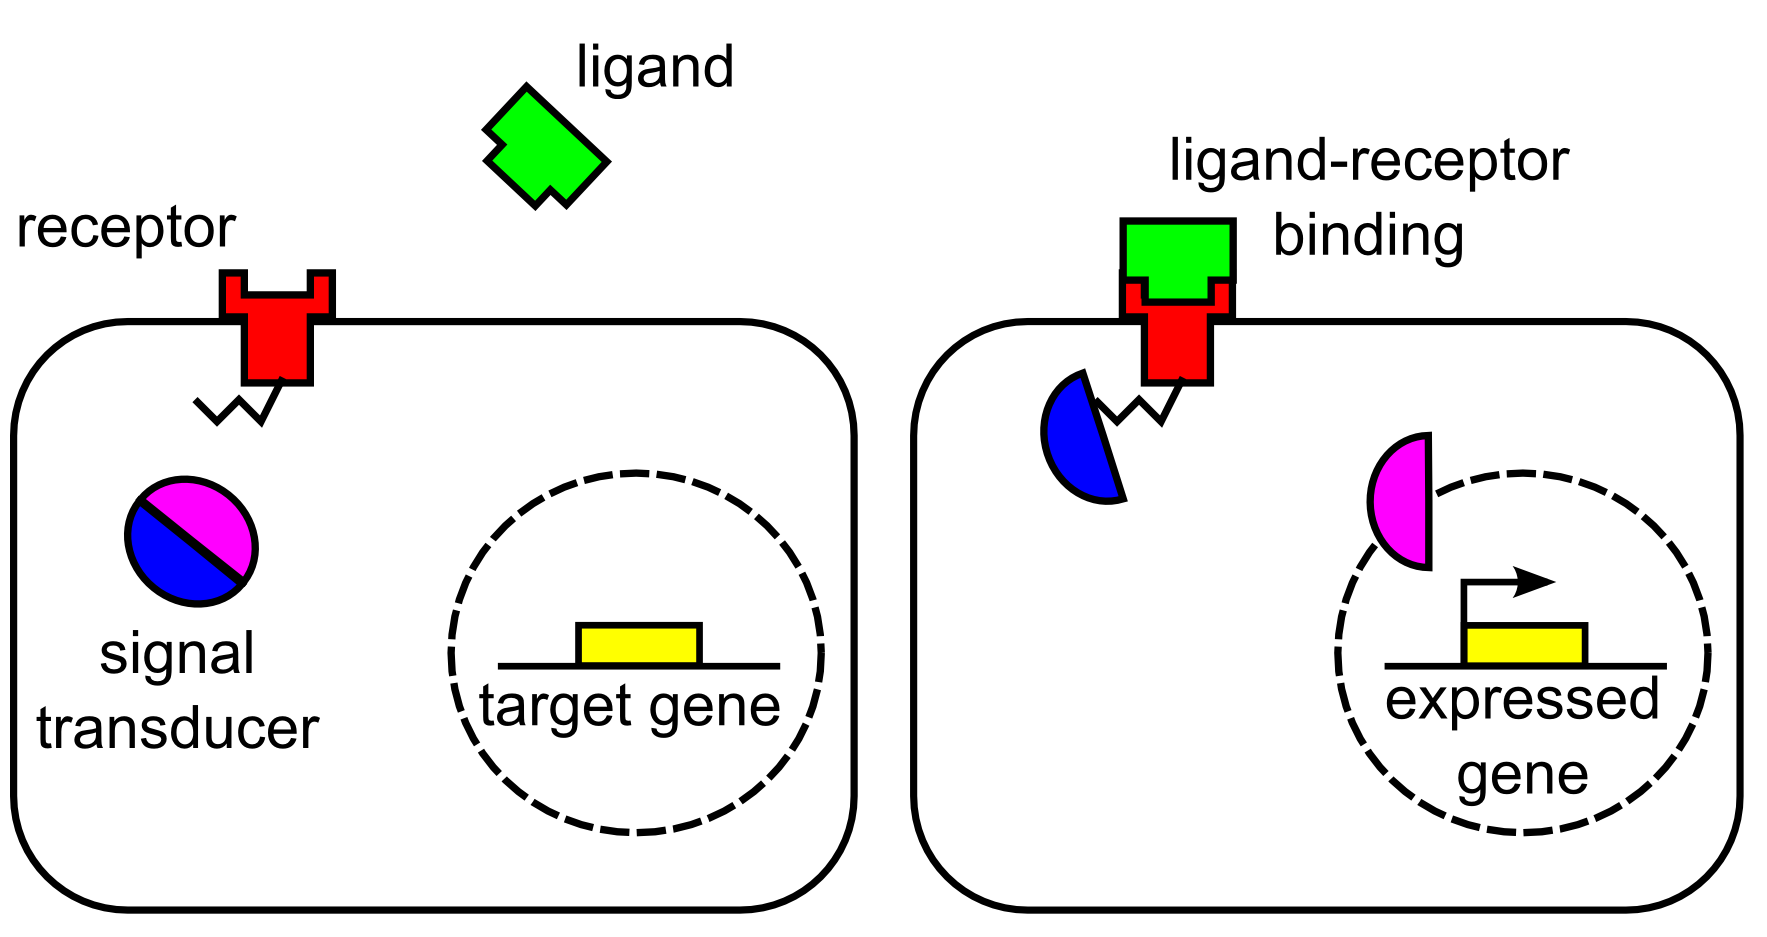
\includegraphics[width=10cm]{./Images/signalling.png}
  \centering
  \caption{
  Scheme of an hypothetical signalling pathway. Left: The extracellular ligand (green) is not bound to the membrane receptor (red) so the signal transducer protein (blue/magenta) is inactivated. In the nucleus (dashed circle) the target gene (yellow box) is inactive. Right: As the ligand binds to the receptor, the cytoplasmic domain (depicted as a zigzag tail) of the receptor change to an active conformation, cleaving the signal transducer. Part of the signal transducer acts as a transcription factor, going into the nucleus where activates the transcription of the target gene after binding to its regulatory region.
 }
  \label{fig:Signalling}
\end{figure}
%%%%%%%%%%%%%%%%%%%%%%%%%%%%%%%%%%%%%%%%%%%%%%%%%%%%%%%%%%%%%%%%%%%%%%%%%%%%%%%%%%%%%

\paragraph{Transcription factors} The transcription factors (TFs) are proteins that bind to specific regulatory regions, to induce or repress the expression of a gene.
Based on the secondary structure of the protein binding domain, TFs can b e classified in four main families: helix-turn-helix, helix-loop-helix, zinc finger and leucine zipper (\citep{Carroll2001}.
	\nomenclature{TF}{Transcription Factor}
	
The members of each family has been recognised in playing different roles in development. For example, it has been observed that in diverse metazoan species C2H2 zinc-figers TFs are over-represented in early development, as opposite to Homeobox TFs which are under-represented in the same period \citep{Schep2013}.
Hox genes (a subset of the Homeobox TF family) are involved in the A/P patterning of many metazoan groups. Intriguingly, these genes were found to have spatial collinearity in mice and flies (REF). That means that the A/P expression of the Hox genes reflects their physical order along the chromosome.
At the time of its discovery, collinearity of Hox genes were considered as a master plan for A/P patterning in animals (REF).
However, after Hox genes were investigated in more species it became clear that in some species with Hox genes collinearity is not always present, and some species do not have Hox genes at all (REF).

\paragraph{Signalling pathway genes} Signalling pathways are usually a complex network of molecules including extracellular diffusible signals, membrane receptors, intermediate signal transducer molecules and transcription factors.
Signalling pathways usually begin with a extracellular signal that causes a conformational change in its cell membrane receptor after binding to it.
The new conformation results in enzymatic activity in the cytoplasmic domains of the receptor protein, that phosphorylate other cytoplasmic proteins.
Finally, one or more activated transcription factors induce or repress specific gene activity \citep{Gilbert2014}.

Signalling pathways recurrently used during animal development are the Wnt, FGF and Shh pathways (for a detailed description of each signalling pathway, see \citep{Gilbert2014}.
For example, the Shh pathway plays a fundamental role in the fruit fly segment polarization(REF) and wing development (REF), and in vertebrate limb (REF) and tooth development \citep{Jernvall2000b}.


\subsection{Complexity Increase in Evolution}

The increase in complexity in evolution has has been a topic of interest for more than a century.
Early views of evolution saw the increase in complexity as inexorable, with all the species descending from simpler ancestral forms \citep{lamarck1809zoo,haeckel1874menschen}, and with the human species as the latest and more perfect product of the evolution of animals \citep{haeckel1874menschen}.


Recent views recognize that within a phylum, complexity of the species can increase or decrease.
Using the number of cell-types as complexity measure, there are clear examples of taxa that have decreased their complexity over time, specially in parasites.
An example would be the animal group formerly known as the "Mesozoa", which are worm-like parasites of marine invertebrates.
Because of their simple morphology (based on their small number of cell types), these animals were thought to be "living fossils" or intermediate forms between Protozoans and Metazoans.
Now, even when they remain poorly studied animals, it is thought that they are degenerate descendants of more complex ancestors, probably some lophotrochozoan group \citep{Arthur2010}.
The Orthonectida, for example, is a phylum of parasites of marine invertebrates with only two types of cells, external ciliated and internal reproductive cells without any internal organs. 
Molecular phylogenetic analysis provided evidence that these animals are more closely related to tripoblastic animals than to protists or diplobastic taxa \citep{Hanelt1996}.
These animals most probably evolved from a more complex free living animal and decreased their morphological complexity after they adopted a parasitic life style.

So, it seems that there is no unique trend to increase the complexity over time, i.e., in a specific lineage, complexity might decrease, increase or stay the same (see Figure \ref{fig:Complexity_min}a).

\subsubsection{Is there a trend towards increasing complexity?}

As the organisms have a wide range of morphological complexities, it is useful to use an statistical approach to identify a trend towards increasing complexity.
If we consider a minimum complexity statistic, it can be said that complexity has remained more or less constant in evolution, as low complexity (unicellular) organisms like bacteria, have been present from 3.5 billion years.

If we look at the mean or maximum statistics, a trend for increasing complexity would be apparent, as the initial complexity would have increased with the appearance of simple multicellular organisms (only few cell types) and would have increase more with the appearance of organisms composed of hundreds of cell types.

It is important to notice that this apparent trend towards increasing complexity does not necessarily imply that it has been selected for \citep{McShea2015}.
Even a "passive" mechanism, 
%in which the organisms increase or decrease their complexity in a process similar to a random walk or diffusion, with a minimum complexity requirement. 
could result in an apparent complexity increase.

In this case, given that the first organisms would have been simple, and there is a low complexity boundary (it is not possible to be simpler than an unicellular organims), even if the complexity of different lineages would have changed in a random walk fashion (see Figure \ref{fig:Complexity_min}b) the mean and maximum complexity would increase in evolution \citep{gould1996fullhouse}.

%McShea has proposed three different mechanisms that would account for the same trend of increasing the mean and maximum complexity: 1) a strongly driven mechanism, 2) a weakly driven mechanism and 3) a Passive

%EXPLAIN MORE ABOUT THE MINIMUM-MEAN-MAX

%However, if we could depict the change in complexity in all lineages (see Figure \ref{fig:Complexity_min}b), we probably would see that the range of complexity has increased over time, with the a lower limit or minimum complexity that has stayed the same and with an increase in mean and maximun (or upper limit) of complexity \citep{McShea1996,Arthur2010}.

%%%%%%%%%%%%%%%%%%%%%%%%%%%%%%%%%%%%%%%%%%%%%%%%%%%%%%%%%%%%%%%%%%%%%%%%%%%%%%%%%%%%%
\begin{figure}[t]
  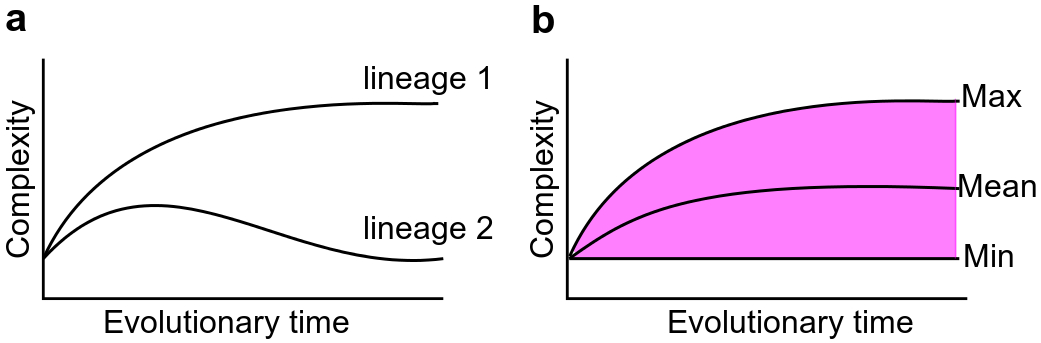
\includegraphics[width=12cm]{./Images/complexity_min.jpeg}
  \centering
  \caption{a) Two lineages with different complexity change through their evolutionary trajectories.
  b) Representation of the minimum, mean and maximum complexity of many lineages over evolutionary time in which the minimum stay constant while the mean and maximum increase.
Redrawn from \citep{Arthur2010}.
 }
  \label{fig:Complexity_min}
\end{figure}
%%%%%%%%%%%%%%%%%%%%%%%%%%%%%%%%%%%%%%%%%%%%%%%%%%%%%%%%%%%%%%%%%%%%%%%%%%%%%%%%%%%%%

%\subsection{Complexity Increase in Development}
%
%The increase in complexity in an organism during embryogenesis is probably one of the most intuitive processes of animal development.
%It is commonly seen even as one of its defining characteristics.
%Eric H. Davidson described the progressive increase in complexity as the "essence" of development \citep{Davidson2001}. Despite of the widely accepted view of complexity increase in development, there is no consensus of how to define it, much less on how to quantify it \citep{susan2000ontogeny}.
%
%Using the number of cell types again as a proxy of morphological complexity, it can be said that during metazoan development, complexity increases as the zygote divides and differentiates into an adult with multiple cell types. 
%This simple definition of complexity has its complications, as there is no clear criteria of how to define a cell type or how to determine when a new cell type has formed during development. 
%For example, it could be that at the morphological level a cell seems to be undifferentiated, but when isolating it from its neighbour cells, it differentiates in an autonomous way into a specific cell type, suggesting that the cell fate was already determined without the necessity of further interactions with other cells.
%
%\textbf{Talk about differentiation and determination?}
%
% 
%In addition, this definition does not take into account that embryos do not only get more cell types, but these cell types become organized in specific patterns in space and time in the embryo, which also could be considered as an increase in complexity over developmental time.

%%%%%%%%%%%%%%%%%%%%%%%%%%%%%%%%%%%%%%%%%%%%%%%%%%%%%%%%%%%%%%%%%%%%%%%%%%%%%%%%%%%%%%
%%\clearpage
%\begin{mdframed}[style=boxstyle,frametitle={Box1. On the similarity of complexity patterns between Evolution and Development}]\label{Box1:Haeckel&vonBaer}
%
%The connection between the increase in complexity during development and evolutionary time it has been largely discussed.
%Haeckel was one of the first who made explicit hypothesis about the connection between the development and evolutionary patterns.
%In what is known as Haeckel's "Biogenetic Law", he described development (or ontogeny), as a brief summary of the slow and long phylogeny \citep{haeckel1874menschen}.
%In his hypothesis, a "higher" organism would pass through a series of conserved developmental stages that represent ancestral forms. This view is also known as the "recapitulation theory".
%
%Karl Ernst von Baer, an Estonian naturalist, also formulated his own hypotheses, known as von Baer's laws \citep{vonBaer1828uber}. He stated that general characteristics develop before special characteristics (first law) and, opposed to Haeckel, that the embryo of a "higher" animal never resembles the adult of another animal form, but only his embryo (fourth law). 
%
%Apart from the differences in the "recapitulation" view, Haeckel and von Baer \citep{Richardson2002} they disagreed in the acceptance of evolution. 
%Haeckel's view was an evolutionary one, while von Baer's was not. Curiously, von Baer's arguments were used by Darwin in its "Origin" \citep{darwin1859origin} to support common ancestry and therefore, evolution.
%
%Now is evident that any of these hypotheses can be considered "laws", as they are not universal. They only apply to some characters, stages and levels of phylogenetic inclusiveness \citep{Richardson2002}. Nevertheless, both Haeckel and von Baer work represented the foundations of the comparative embryology field, which is in turn the basis of the modern evolutionary developmental biology (evo-devo).
%	\nomenclature{Evo-devo}{Evolutionary Developmental Biology}
%\end{mdframed}
%%%%%%%%%%%%%%%%%%%%%%%%%%%%%%%%%%%%%%%%%%%%%%%%%%%%%%%%%%%%%%%%%%%%%%%%%%%%%%%%%%%%%%

\subsection{Other definitions of complexity}


\subsubsection{Complexity in informational terms}

\cite{Davidson2001} used the GRN concept in addition to others to explain development (and evolution) on informational terms. He said that development (which is the outcome of spatial and temporal series of differential gene expression) is controlled by a hardwired regulatory program built into the DNA and the metric of complexity is the diversity of the programs of gene expression that are "installed and executed" as the embryo develops. As Davidson, other authors have used informational/computational analogies to define development \citep{Apter1965,monod2012cytodifferentiation,mayr1997evolution} 

To illustrate how the complexity of a regulatory network or "program" can increase in evolution (but a similar case could be said for development), Davidson describes an imaginary example:
an early evolutionary state consists of a small gene battery (set of functionally linked genes expressed in concert) encoding proteins used for some differentiated cell type, which is activated by a small number of genes encoding transcription factors. The network activating the gene battery is itself controlled by a single upstream gene.
In subsequent evolutionary states, the whole structure is said to become more complex as: the battery of genes is now used in some pattern formation system, new batteries of genes appear, new regulatory genes and new \textit{cis}-regulatory regions are introduced  \citep{Davidson2001}.

Even when in this kind of examples would seem easy to discern a simple GRN from a complex one just from its topology, the high intricacy of real biological systems make this an extremely difficult if not impossible task. 

%%%%%%%%%%%%%%%%%%%%%%%%%%%%%%%%%%%%%%%%%%%%%%%%%%%%%%%%%%%%%%%%%%%%%%%%%%%%%%%%%%%%%
\begin{figure}[h]
  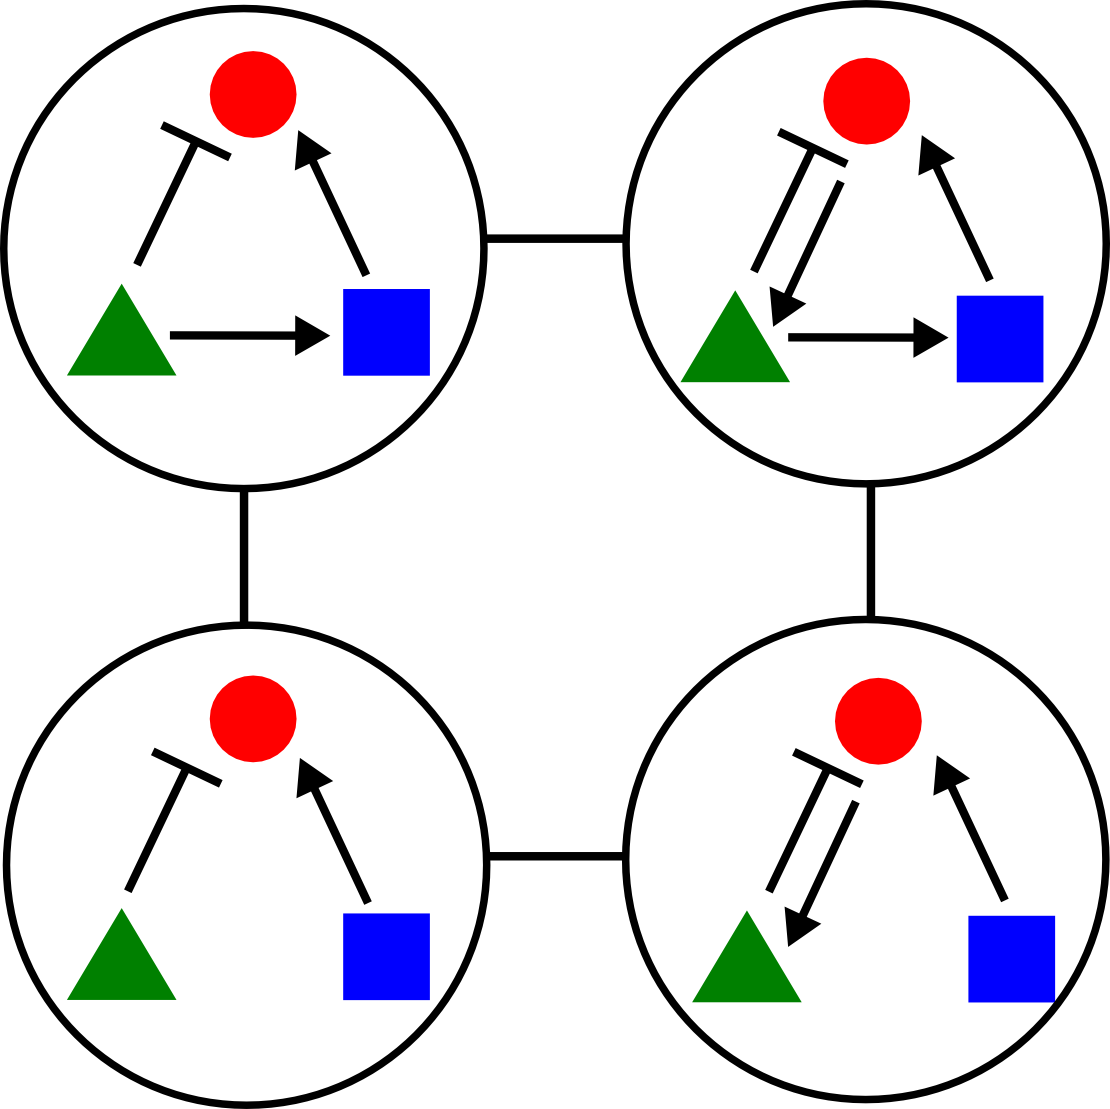
\includegraphics[width=5cm]{./Images/GRNs.png}
  \centering
  \caption{
  Some GRNs . Cotterel and Harpe calculated... \citep{Cotterell2010}
 }
  \label{fig:GRNs}
\end{figure}
%%%%%%%%%%%%%%%%%%%%%%%%%%%%%%%%%%%%%%%%%%%%%%%%%%%%%%%%%%%%%%%%%%%%%%%%%%%%%%%%%%%%%

There are also important critiques of this informational approach. First, using an informational analogy to describe development implies the distinction between a "hardware" and a "software".
The "hardware" would consist of the genome structure, regulatory components, cells, organs, etc., and the "software" would be the GRNs or the set of instructions that directs the performance of specific operations.
For biological systems, this distinction is misleading, as there are recurrent feedback between its "hardware" and "software", so that the structure of development processes change through development \citep{susan2000ontogeny,Salazar-Ciudad2009,Jaeger2014devmech}.


\subsubsection{Complexity in terms of dynamical systems theory}

Estimating the combinatorial possibilities of a small set of regulatory genes, considering that each gene can regulate (whether positively or negatively) more than one gene's expression in addition to its own, could result in an astronomic number of possible gene topologies (see Figure \ref{fig:GRNs}).
Also feedback effects and non-linear regulation of gene expression make the prediction of changes in regulatory states hard or even impossible to predict \citep{Jaeger2014devmech}.

To overcome this limitations, some authors have propose to use dynamical systems theory, which deals with a complex system with many interacting components (a dynamical system), by representing its state as a point in a multidimensional space \citep{Alberch1991,ForgacsandStuartA.Newman.2005,Jaeger2014devmech}. 
To illustrate this we could think of a specific cell type, with \textit{n} number of genes, which its cell state depends on the expression of each of the genes.
The simpler case we could imagine would be a cell with only two genes. In this case, the cell would be in a two-dimensional "state space" (also called "phase space").

Importantly, the dynamical system is governed by the relations between its components \citep{ForgacsandStuartA.Newman.2005}. In our example the relations would be represented by the interaction between genes, namely the gene regulatory network (GRN). 
If in our example the expression level of one gene is affected by the expression level of the other gene, the system will not stay in any particular state, but it will change until it reaches a "stable steady state", in which the level of both genes are at equilibrium. 
Given a specific GRN, the number of stable states would represent the possible differentiation states a cell can achieve (REF Slack book)

Many modifications of the GRN would not have consequences in the ultimate differentiation state, as it will converge to the same "attractor" point.
However, some modifications (or mutations) could produce a change in the "state space" leading to the formation of a new stable state (i.e., a new cell type).
So within the framework of the dynamical systems theory, and keeping the number of cell types as our measure of complexity, there would be an increase in complexity when a mutation would change the gene regulatory machinery so that a new stable steady state is formed.


%\textbf{Make a figure?}
%-nothing about spatial or statistical approach like our disparity measure
%- explain something about non-genetic components? (Newman, Gabor and Forgacs, Alberch, Isaac)

%\clearpage